% Generated by Sphinx.
\def\sphinxdocclass{report}
\documentclass[letterpaper,10pt,openany,oneside]{sphinxmanual}
\usepackage[utf8]{inputenc}
\DeclareUnicodeCharacter{00A0}{\nobreakspace}
\usepackage[T1]{fontenc}
\usepackage[english]{babel}
\usepackage{times}
\usepackage[Bjarne]{fncychap}
\usepackage{longtable}
\usepackage{sphinx}
\usepackage{multirow}


\title{Map-reduce Computing for Introductory Students using WebMapReduce}
\date{October 26, 2012}
\release{}
\author{CSInParallel Project}
\newcommand{\sphinxlogo}{}
\renewcommand{\releasename}{}
\makeindex

\makeatletter
\def\PYG@reset{\let\PYG@it=\relax \let\PYG@bf=\relax%
    \let\PYG@ul=\relax \let\PYG@tc=\relax%
    \let\PYG@bc=\relax \let\PYG@ff=\relax}
\def\PYG@tok#1{\csname PYG@tok@#1\endcsname}
\def\PYG@toks#1+{\ifx\relax#1\empty\else%
    \PYG@tok{#1}\expandafter\PYG@toks\fi}
\def\PYG@do#1{\PYG@bc{\PYG@tc{\PYG@ul{%
    \PYG@it{\PYG@bf{\PYG@ff{#1}}}}}}}
\def\PYG#1#2{\PYG@reset\PYG@toks#1+\relax+\PYG@do{#2}}

\expandafter\def\csname PYG@tok@gd\endcsname{\def\PYG@tc##1{\textcolor[rgb]{0.63,0.00,0.00}{##1}}}
\expandafter\def\csname PYG@tok@gu\endcsname{\let\PYG@bf=\textbf\def\PYG@tc##1{\textcolor[rgb]{0.50,0.00,0.50}{##1}}}
\expandafter\def\csname PYG@tok@gt\endcsname{\def\PYG@tc##1{\textcolor[rgb]{0.00,0.25,0.82}{##1}}}
\expandafter\def\csname PYG@tok@gs\endcsname{\let\PYG@bf=\textbf}
\expandafter\def\csname PYG@tok@gr\endcsname{\def\PYG@tc##1{\textcolor[rgb]{1.00,0.00,0.00}{##1}}}
\expandafter\def\csname PYG@tok@cm\endcsname{\let\PYG@it=\textit\def\PYG@tc##1{\textcolor[rgb]{0.25,0.50,0.56}{##1}}}
\expandafter\def\csname PYG@tok@vg\endcsname{\def\PYG@tc##1{\textcolor[rgb]{0.73,0.38,0.84}{##1}}}
\expandafter\def\csname PYG@tok@m\endcsname{\def\PYG@tc##1{\textcolor[rgb]{0.13,0.50,0.31}{##1}}}
\expandafter\def\csname PYG@tok@mh\endcsname{\def\PYG@tc##1{\textcolor[rgb]{0.13,0.50,0.31}{##1}}}
\expandafter\def\csname PYG@tok@cs\endcsname{\def\PYG@tc##1{\textcolor[rgb]{0.25,0.50,0.56}{##1}}\def\PYG@bc##1{\setlength{\fboxsep}{0pt}\colorbox[rgb]{1.00,0.94,0.94}{\strut ##1}}}
\expandafter\def\csname PYG@tok@ge\endcsname{\let\PYG@it=\textit}
\expandafter\def\csname PYG@tok@vc\endcsname{\def\PYG@tc##1{\textcolor[rgb]{0.73,0.38,0.84}{##1}}}
\expandafter\def\csname PYG@tok@il\endcsname{\def\PYG@tc##1{\textcolor[rgb]{0.13,0.50,0.31}{##1}}}
\expandafter\def\csname PYG@tok@go\endcsname{\def\PYG@tc##1{\textcolor[rgb]{0.19,0.19,0.19}{##1}}}
\expandafter\def\csname PYG@tok@cp\endcsname{\def\PYG@tc##1{\textcolor[rgb]{0.00,0.44,0.13}{##1}}}
\expandafter\def\csname PYG@tok@gi\endcsname{\def\PYG@tc##1{\textcolor[rgb]{0.00,0.63,0.00}{##1}}}
\expandafter\def\csname PYG@tok@gh\endcsname{\let\PYG@bf=\textbf\def\PYG@tc##1{\textcolor[rgb]{0.00,0.00,0.50}{##1}}}
\expandafter\def\csname PYG@tok@ni\endcsname{\let\PYG@bf=\textbf\def\PYG@tc##1{\textcolor[rgb]{0.84,0.33,0.22}{##1}}}
\expandafter\def\csname PYG@tok@nl\endcsname{\let\PYG@bf=\textbf\def\PYG@tc##1{\textcolor[rgb]{0.00,0.13,0.44}{##1}}}
\expandafter\def\csname PYG@tok@nn\endcsname{\let\PYG@bf=\textbf\def\PYG@tc##1{\textcolor[rgb]{0.05,0.52,0.71}{##1}}}
\expandafter\def\csname PYG@tok@no\endcsname{\def\PYG@tc##1{\textcolor[rgb]{0.38,0.68,0.84}{##1}}}
\expandafter\def\csname PYG@tok@na\endcsname{\def\PYG@tc##1{\textcolor[rgb]{0.25,0.44,0.63}{##1}}}
\expandafter\def\csname PYG@tok@nb\endcsname{\def\PYG@tc##1{\textcolor[rgb]{0.00,0.44,0.13}{##1}}}
\expandafter\def\csname PYG@tok@nc\endcsname{\let\PYG@bf=\textbf\def\PYG@tc##1{\textcolor[rgb]{0.05,0.52,0.71}{##1}}}
\expandafter\def\csname PYG@tok@nd\endcsname{\let\PYG@bf=\textbf\def\PYG@tc##1{\textcolor[rgb]{0.33,0.33,0.33}{##1}}}
\expandafter\def\csname PYG@tok@ne\endcsname{\def\PYG@tc##1{\textcolor[rgb]{0.00,0.44,0.13}{##1}}}
\expandafter\def\csname PYG@tok@nf\endcsname{\def\PYG@tc##1{\textcolor[rgb]{0.02,0.16,0.49}{##1}}}
\expandafter\def\csname PYG@tok@si\endcsname{\let\PYG@it=\textit\def\PYG@tc##1{\textcolor[rgb]{0.44,0.63,0.82}{##1}}}
\expandafter\def\csname PYG@tok@s2\endcsname{\def\PYG@tc##1{\textcolor[rgb]{0.25,0.44,0.63}{##1}}}
\expandafter\def\csname PYG@tok@vi\endcsname{\def\PYG@tc##1{\textcolor[rgb]{0.73,0.38,0.84}{##1}}}
\expandafter\def\csname PYG@tok@nt\endcsname{\let\PYG@bf=\textbf\def\PYG@tc##1{\textcolor[rgb]{0.02,0.16,0.45}{##1}}}
\expandafter\def\csname PYG@tok@nv\endcsname{\def\PYG@tc##1{\textcolor[rgb]{0.73,0.38,0.84}{##1}}}
\expandafter\def\csname PYG@tok@s1\endcsname{\def\PYG@tc##1{\textcolor[rgb]{0.25,0.44,0.63}{##1}}}
\expandafter\def\csname PYG@tok@gp\endcsname{\let\PYG@bf=\textbf\def\PYG@tc##1{\textcolor[rgb]{0.78,0.36,0.04}{##1}}}
\expandafter\def\csname PYG@tok@sh\endcsname{\def\PYG@tc##1{\textcolor[rgb]{0.25,0.44,0.63}{##1}}}
\expandafter\def\csname PYG@tok@ow\endcsname{\let\PYG@bf=\textbf\def\PYG@tc##1{\textcolor[rgb]{0.00,0.44,0.13}{##1}}}
\expandafter\def\csname PYG@tok@sx\endcsname{\def\PYG@tc##1{\textcolor[rgb]{0.78,0.36,0.04}{##1}}}
\expandafter\def\csname PYG@tok@bp\endcsname{\def\PYG@tc##1{\textcolor[rgb]{0.00,0.44,0.13}{##1}}}
\expandafter\def\csname PYG@tok@c1\endcsname{\let\PYG@it=\textit\def\PYG@tc##1{\textcolor[rgb]{0.25,0.50,0.56}{##1}}}
\expandafter\def\csname PYG@tok@kc\endcsname{\let\PYG@bf=\textbf\def\PYG@tc##1{\textcolor[rgb]{0.00,0.44,0.13}{##1}}}
\expandafter\def\csname PYG@tok@c\endcsname{\let\PYG@it=\textit\def\PYG@tc##1{\textcolor[rgb]{0.25,0.50,0.56}{##1}}}
\expandafter\def\csname PYG@tok@mf\endcsname{\def\PYG@tc##1{\textcolor[rgb]{0.13,0.50,0.31}{##1}}}
\expandafter\def\csname PYG@tok@err\endcsname{\def\PYG@bc##1{\setlength{\fboxsep}{0pt}\fcolorbox[rgb]{1.00,0.00,0.00}{1,1,1}{\strut ##1}}}
\expandafter\def\csname PYG@tok@kd\endcsname{\let\PYG@bf=\textbf\def\PYG@tc##1{\textcolor[rgb]{0.00,0.44,0.13}{##1}}}
\expandafter\def\csname PYG@tok@ss\endcsname{\def\PYG@tc##1{\textcolor[rgb]{0.32,0.47,0.09}{##1}}}
\expandafter\def\csname PYG@tok@sr\endcsname{\def\PYG@tc##1{\textcolor[rgb]{0.14,0.33,0.53}{##1}}}
\expandafter\def\csname PYG@tok@mo\endcsname{\def\PYG@tc##1{\textcolor[rgb]{0.13,0.50,0.31}{##1}}}
\expandafter\def\csname PYG@tok@mi\endcsname{\def\PYG@tc##1{\textcolor[rgb]{0.13,0.50,0.31}{##1}}}
\expandafter\def\csname PYG@tok@kn\endcsname{\let\PYG@bf=\textbf\def\PYG@tc##1{\textcolor[rgb]{0.00,0.44,0.13}{##1}}}
\expandafter\def\csname PYG@tok@o\endcsname{\def\PYG@tc##1{\textcolor[rgb]{0.40,0.40,0.40}{##1}}}
\expandafter\def\csname PYG@tok@kr\endcsname{\let\PYG@bf=\textbf\def\PYG@tc##1{\textcolor[rgb]{0.00,0.44,0.13}{##1}}}
\expandafter\def\csname PYG@tok@s\endcsname{\def\PYG@tc##1{\textcolor[rgb]{0.25,0.44,0.63}{##1}}}
\expandafter\def\csname PYG@tok@kp\endcsname{\def\PYG@tc##1{\textcolor[rgb]{0.00,0.44,0.13}{##1}}}
\expandafter\def\csname PYG@tok@w\endcsname{\def\PYG@tc##1{\textcolor[rgb]{0.73,0.73,0.73}{##1}}}
\expandafter\def\csname PYG@tok@kt\endcsname{\def\PYG@tc##1{\textcolor[rgb]{0.56,0.13,0.00}{##1}}}
\expandafter\def\csname PYG@tok@sc\endcsname{\def\PYG@tc##1{\textcolor[rgb]{0.25,0.44,0.63}{##1}}}
\expandafter\def\csname PYG@tok@sb\endcsname{\def\PYG@tc##1{\textcolor[rgb]{0.25,0.44,0.63}{##1}}}
\expandafter\def\csname PYG@tok@k\endcsname{\let\PYG@bf=\textbf\def\PYG@tc##1{\textcolor[rgb]{0.00,0.44,0.13}{##1}}}
\expandafter\def\csname PYG@tok@se\endcsname{\let\PYG@bf=\textbf\def\PYG@tc##1{\textcolor[rgb]{0.25,0.44,0.63}{##1}}}
\expandafter\def\csname PYG@tok@sd\endcsname{\let\PYG@it=\textit\def\PYG@tc##1{\textcolor[rgb]{0.25,0.44,0.63}{##1}}}

\def\PYGZbs{\char`\\}
\def\PYGZus{\char`\_}
\def\PYGZob{\char`\{}
\def\PYGZcb{\char`\}}
\def\PYGZca{\char`\^}
\def\PYGZam{\char`\&}
\def\PYGZlt{\char`\<}
\def\PYGZgt{\char`\>}
\def\PYGZsh{\char`\#}
\def\PYGZpc{\char`\%}
\def\PYGZdl{\char`\$}
\def\PYGZti{\char`\~}
% for compatibility with earlier versions
\def\PYGZat{@}
\def\PYGZlb{[}
\def\PYGZrb{]}
\makeatother

\begin{document}

\maketitle
\tableofcontents
\phantomsection\label{index::doc}



\chapter{Using Parallelism to Analyze Very Large Files: Google's Map Reduce Paradigm}
\label{MapReduceIntro/MapReduceIntro:map-reduce-computing-for-introductory-students-using-webmapreduce}\label{MapReduceIntro/MapReduceIntro::doc}\label{MapReduceIntro/MapReduceIntro:using-parallelism-to-analyze-very-large-files-google-s-map-reduce-paradigm}

\section{Introduction}
\label{MapReduceIntro/MapReduceIntro:introduction}
Up to now in this course, you have been writing programs that run
\emph{sequentially} by executing one step at a time until they complete
(unless you mistakenly wrote one with an infinite loop!).
Sequential execution is the standard basic mode of operation on all
computers. However, when we need to process large amounts of data
that might take a long time to complete, we can use a technique
known as \emph{parallel computing}, in which we define portions of our
computation to run at the same time by using multiple processors on
a single machine or multiple computers at the same time.

In a lab and homework in this course you will use a system called
\emph{MapReduce} that was designed to harness the power of many
computers together in a \emph{cluster} to execute in parallel to process
large amounts of data. You will be writing programs designed to run
in parallel, or concurrently (at the same time), each one working
on a portion of the data. By doing this, your parallel program will
be faster than a corresponding sequential version using one
computer to process all of the data. We call this kind of program
one that uses \emph{data parallelism}, because the data is split and
processed in parallel.

\emph{MapReduce} is a strategy for solving problems using two stages for
processing data that includes a sort action between those two
stages. This problem-solving strategy has been used for decades in
\emph{functional programming} languages such as LISP or Scheme. More
recently Google has adapted the map-reduce programming model
(\href{http://labs.google.com/papers/mapreduce.html}{Dean and Ghemawat,2004})
to function efficiently on large clusters of computers to process
vast amounts of data--for example, Google's selection of the entire
web.

The Apache Foundation provides an open-source implementation of
MapReduce for clusters called
\href{http://hadoop.apache.org/core/}{Hadoop}, which has primarily
been implemented by Yahoo!. Student researchers at St. Olaf College
have created a user interface called \emph{WebMapReduce (WMR)} that uses
Hadoop to make map-reduce programming convenient enough for
students in computer science courses to use.


\section{Description of the MapReduce programming model}
\label{MapReduceIntro/MapReduceIntro:description-of-the-mapreduce-programming-model}
In map-reduce programming, a programmer provides two functions,
called the \emph{mapper} and the \emph{reducer}, for carrying out a sequence
of two computational stages on potentially vast quantities of data.
A series of identical `map' functions can be run on a large amount
of input data in parallel, as shown in Figure mrconcept. The
results from these mapper processes, spread across many computers,
are then sent to reduce functions, also spread across many
computers. The most important concepts to remember are these:
\begin{itemize}
\item {} 
The mapper function that you design is applied to each line of
data, and breaks up that data into labelled units of interest,
called \emph{key-value pairs}.

\item {} 
The reducer function that you design is then applied to all the
key-value pairs \emph{that share the same key}, allowing some kind of
consolidation of those pairs.

\end{itemize}
\begin{figure}[htbp]
\centering
\capstart

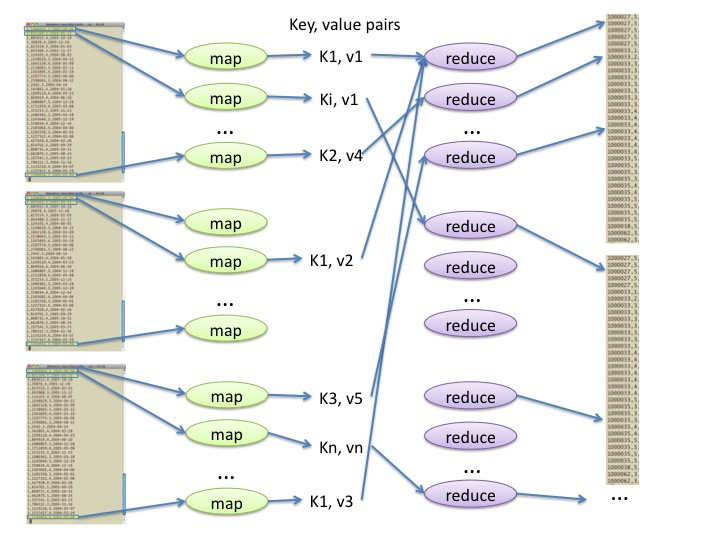
\includegraphics{Figure1.jpg}
\caption{Figure 1: The concept behind how map functions can run in parallel and
pass their results to reduce functions, whose results are output in
sorted order by the keys created by the reduce function.(mrconcept)}\end{figure}

In a \emph{map-reduce system}, which is made of of many computers
working at the same time, some computers are assigned mapper tasks,
some shuffle the data from mappers and hand it over to reducers,
and some computers handle the reducer tasks. Between the mapper and
reducer stages, a map-reduce system automatically reorganizes the
intermediate key-value pairs, so that each call of the reducer
function can receive a complete set of key-value pairs
\emph{for a particular key}, and so that the reducer function is called
for every key in sorted order. We will refer to this reorganization
of key-value pairs between the mapper and reducer stages as
\emph{shuffling}. Figure mrstages illustrates the three steps of
mapping, shuffling, and reducing.
\begin{figure}[htbp]
\centering
\capstart

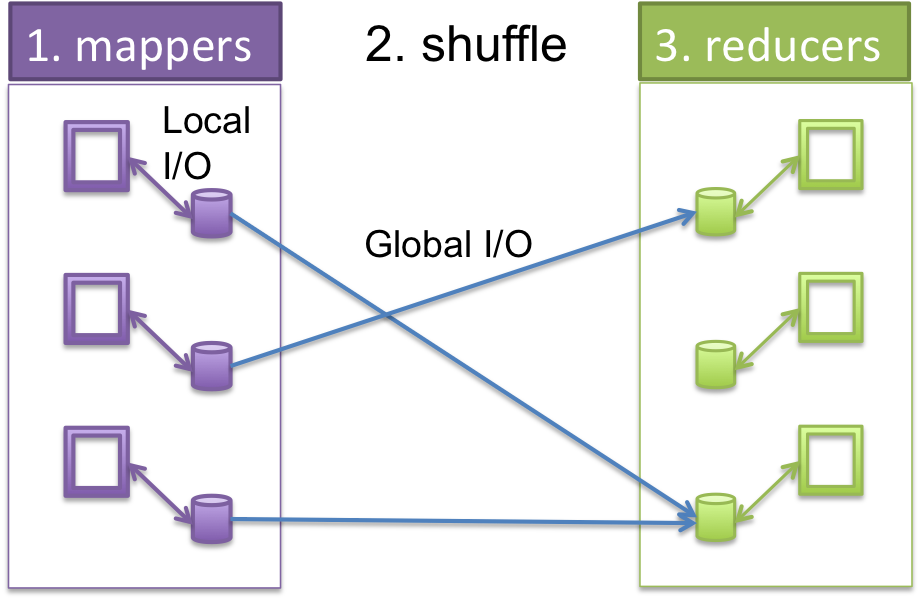
\includegraphics{Figure2.png}
\caption{Figure 2: How each computer in a cluster breaks up the work and runs
mappers locally, then shuffles the key-value pair results by key and
sends the results for each key to other computers who run reducers.(mrstages)}\end{figure}

Before the mapper stage, a map-reduce system such as Hadoop breaks
the entire input data up into portions, known as \emph{splits}; each
split is assigned to one computer in a cluster, which then applies
the mapper function to each line of that split. Thus,multiple
computers can process different splits of data simultaneously.
(With, say, 2000 computers or \emph{nodes} in a large-scale commercial
cluster, quadrillions of bytes (\emph{petabytes}) of data might be
processed in a few hours that might otherwise require years of
computing time on a single computer.) Likewise, reducers may be run
on multiple computers in order to speed up the performance of that
stage.

\emph{Parallel computing} is the practice of using multiple computations
at the same time in order to improve the performance of those
computations. The map-reduce programming model is an example of two
varieties of parallel computing:
\begin{enumerate}
\item {} 
\emph{Data parallelism}, in which multiple portions of data are
processed simultaneously on multiple processors (CPUs). This occurs
when multiple splits of data are handled on different computers in
a cluster.

\item {} 
\emph{Pipelining}, in which data is processed in a sequence of
stages, like an assembly line. The mapper and reducer stages
represent a two-stage pipeline. If shuffling is considered as its
own stage, the pipeline would have three stages. Pipelining is an
example of \emph{task parallelism}, in which different computational
tasks take place at the same time. In the case of the map-reduce
stages, mapping could overlap with shuffling to some extent, by
having mappers stream their output to shuffle processes, which
would prepare it for reducers while the mappers are generating
results. Thus, different computers could handle each of these
tasks.

\end{enumerate}

\begin{notice}{note}{Note:}
Hadoop actually carries out the three stages of mapping,
shuffling, and reducing \emph{sequentially} (one stage after the other),
instead of using task parallelism. That is, all of the mapping
occurs before any of the shuffling begins, and all of the shuffling
is completed before any of the reducing begins. (See below for
reasons why.) Thus, Hadoop's implementation of map-reduce doesn't
literally qualify as pipeline parallelism, because multiple stages
do not take place at the same time. However, true pipeline
parallelism \emph{does} take place within our testing program used in
the \code{WebMapReduce} interface, called \code{wmrtest}, which is useful
for testing and debugging mapper and reducer functions with small
data. In general, solving problems using pipeline (assembly line)
thinking creates opportunities for using parallelism to improve
performance.
\end{notice}

\textbf{Fault tolerance.} Large (e.g., 2000-node) clusters offer the
potential for great performance speedup, but breakdowns are
inevitable when using so many computers. In order to avoid losing
the results of enormous computations because of breakdowns,
map-reduce systems such as Hadoop are \emph{fault tolerant}, i.e.,
designed to recover from a significant amount of computer failure.
Here are some fault-tolerance strategies used in Hadoop:
\begin{itemize}
\item {} 
All data is \emph{replicated} on multiple computers. Thus,if one
computer fails, its data is readily available on other computers.

\item {} 
If a computer running a mapper function fails, that mapper
operation can thus be restarted on another computer that has the
same data (after discarding the partial results (key-value pairs)
from incomplete mapper calls on that failed computer).

\item {} 
If all mappers have completed, but a computer fails during
shuffling, then any lost mapper results can be regenerated on
another computer, and shuffling can resume using non-failed
computers.

\item {} 
Shuffling results are also replicated, so if a computer running
reducers fails, those reducers can be rerun on another computer.

\end{itemize}

\begin{notice}{note}{Note:}
Hadoop's fault tolerance features make it a good use for
the \emph{selkie} cluster at Macalester, which uses the many computers
in two large labs in the MSCS Department in Olin-Rice.
Occasionally, these are sometimes unfortunately rebooted by users.
These occasional failures of machines in the cluster can be
compensated for by Hadoop. However, when many of these computers
are rebooted at about the same time, all of the copies of some data
may become unavailable, leading to Hadoop failures.
\end{notice}


\chapter{Using WebMapReduce (WMR)}
\label{wmr_py/wmr_py:using-webmapreduce-wmr}\label{wmr_py/wmr_py::doc}

\section{Introduction}
\label{wmr_py/wmr_py:introduction}
For this activity, you need to have read the accompanying
background reading entitled
\emph{Using Parallelism to Analyze Very Large Files: Google's MapReduce Paradigm}.

In this lab you will use a web-based program called \emph{WebMapReduce}
(\textbf{WMR}) that enables you to formulate map-reduce computations and
run them on an underlying \emph{Hadoop} map-reduce system running on a
cluster of computers.

You will use WebMapReduce on a cluster of computers at Macalester
College. You should access WebMapReduce now and register for a
login by going to this URL on your web browser:

\href{http://selkie.macalester.edu/wmr}{http://selkie.macalester.edu/wmr}

Choose the link at the very upper right of this page that says
`Register'. Use your Macalester email address as your login name,
and provide the other information asked for. You choose your own
password, so that you can remember it and have control of your
account.

WMR has several languages as options, and Python is one of them,
although it expects Python3. Though we have been using Python 2.7
in our class, the difference for the following example is really
close to what you have already used. We will highlight the
difference below.

For later reference, you may want to check this documentation for
WMR:

\href{http://webmapreduce.sourceforge.net/docs/User\_Guide/index.html}{http://webmapreduce.sourceforge.net/docs/User\_Guide/index.html}

This WMR user guide has images from the first version of WMR, but a
great deal of the information about how to use it remains the same.
For this activity, you should be able to follow along with the
instructions and determine how to use WMR.


\section{An example of map-reduce computing with WMR: counting words}
\label{wmr_py/wmr_py:an-example-of-map-reduce-computing-with-wmr-counting-words}
To program with map-reduce, you must first decide how to use
mappers and reducers in order to accomplish your computational
goal. The mapper function should take a line of input and decompose
it somehow into key-value pairs; then the reducer should somehow
condense or analyze all the key-value pairs having a common key,
and produce a desired result.

\emph{The following example is small to illustrate how the process works.}
In realistic applications, which you will try later in this
activity and in homework, the input data is much larger (several to
hundreds of Gigabytes) and is stored in the Hadoop system. You will
go through the following exercise first to ensure that the code is
working and that you understand how it works. Then you can move on
to bigger files. This is the process you should go through when
doing this kind of coding: work on small amounts of data first to
ensure correctness of your code, then try larger amounts of data.

As an example, consider the problem of counting how frequently each
word appears in a collection of data. For example, if the input
data in a file is:

\begin{Verbatim}[commandchars=\\\{\}]
One fish, Two fish,
Red fish, Blue fish.
\end{Verbatim}

then the output should be:

\begin{Verbatim}[commandchars=\\\{\}]
Blue 1
One 1
Red 1
Two 1
fish, 3
fish. 1
\end{Verbatim}

As this output indicates, we did not make any attempt to trim
punctuation characters in this first example. We will do so as we
practice using WebMapReduce with the initial functions described
below. (Note that the WebMapReduce system will sort the words
according to the ASCII codes of the characters within words.)

What follows is a plan for the mapper and reducer functions. You
should compare and note the similarity between these and your
sequential function for completing this same task on a single input
file.


\subsection{Map-reduce plan}
\label{wmr_py/wmr_py:map-reduce-plan}
In WMR, mapper functions work simultaneously on lines of input from
files, where a line ends with a newline charater. The mapper will
produce one key-value pair (\emph{w}, \emph{count}) foreach word encountered
in the input line that it is working on.

Thus, on the above input, two mappers working together on each line
would emit the following combined output:

\begin{Verbatim}[commandchars=\\\{\}]
One 1
fish, 2
Two 1
Red 1
fish, 1
Blue 1
fish. 1
\end{Verbatim}

The reducers will compute the sum of all the \emph{count} values for a
given word \emph{w}, then produce the key-value pair (\emph{w}, \emph{sum}).


\section{The mapper function}
\label{wmr_py/wmr_py:the-mapper-function}
Here is a Python3 mapper function for accomplishing this task using
the WMR system. We also add the feature of stripping away
puncuation characters from the input.

\begin{Verbatim}[commandchars=\\\{\}]
\PYG{k+kn}{import} \PYG{n+nn}{string}

\PYG{k}{def} \PYG{n+nf}{mapper}\PYG{p}{(}\PYG{n}{key}\PYG{p}{,} \PYG{n}{value}\PYG{p}{)}\PYG{p}{:}
    \PYG{n}{counts} \PYG{o}{=} \PYG{n+nb}{dict}\PYG{p}{(}\PYG{p}{)}  \PYG{c}{\PYGZsh{}create a dictionary to hold words}
    \PYG{n}{words}\PYG{o}{=}\PYG{n}{key}\PYG{o}{.}\PYG{n}{split}\PYG{p}{(}\PYG{p}{)}
    \PYG{k}{for} \PYG{n}{word} \PYG{o+ow}{in} \PYG{n}{words}\PYG{p}{:}
        \PYG{n}{word} \PYG{o}{=} \PYG{n}{word}\PYG{o}{.}\PYG{n}{strip}\PYG{p}{(}\PYG{n}{string}\PYG{o}{.}\PYG{n}{punctuation}\PYG{p}{)}
        \PYG{k}{if} \PYG{n}{word} \PYG{o+ow}{not} \PYG{o+ow}{in} \PYG{n}{counts}\PYG{p}{:}
            \PYG{n}{counts}\PYG{p}{[}\PYG{n}{word}\PYG{p}{]} \PYG{o}{=} \PYG{l+m+mi}{1}
        \PYG{k}{else}\PYG{p}{:}
            \PYG{n}{counts}\PYG{p}{[}\PYG{n}{word}\PYG{p}{]} \PYG{o}{+}\PYG{o}{=} \PYG{l+m+mi}{1}

    \PYG{k}{for} \PYG{n}{foundword} \PYG{o+ow}{in} \PYG{n}{counts}\PYG{p}{:}
        \PYG{n}{Wmr}\PYG{o}{.}\PYG{n}{emit}\PYG{p}{(}\PYG{n}{foundword}\PYG{p}{,} \PYG{n}{counts}\PYG{p}{[}\PYG{n}{foundword}\PYG{p}{]}\PYG{p}{)}
\end{Verbatim}

This code is available \code{for download as wc\_comb\_mapper.py}.
You can use this file later when you wish to use it as your mapper in WMR.

Let's examine this code carefully. In line 1 we import the Python
\code{string} package so that we can use its method for returning
punctuation characters, found in line 7. Line 3 shows how all
mapper functions in WMR should be defined, with two parameters
called \emph{key} and \emph{value}. Each of these parameters is a \emph{String}
data type. In the case of our first mapper functions reading each
line of the file, the whole line is passed into the key in the
map-reduce system underlying WMR, and the value is empty. (See
additional notes section below for more details you will need when
trying other examples.)

In line 4, we create a Python dictionary called \emph{counts} to hold
each distinct word and the number of time it appears. In the small
input example we describe here, this will not have many entries.
When we next read files where a whole book may be contained in one
line of data, the dictionary called counts will contain many
words.

Line 5 is where we take the input line, which was in the \emph{key}, and
break it into words. Then the loop in lines 6-11 goes word by word
and strips punctuation and increments the count of that word.

The loop in lines 13 and 14 is how we send the data off to the
reducers. The WMR system for Python3 defines a class \code{Wmr{}`{}`that
includes a class method {}`{}`emit()} for producing key-value pairs to
be forwarded (via shuffling) to a reducer. \code{Wmr.emit()} requires
two string arguments, so both \emph{foundword} and \emph{counts{[}foundword{]}}
are being interpreted as strings in line 14.


\section{The reducer function}
\label{wmr_py/wmr_py:the-reducer-function}
A reducer function for solving the word-count problem is
\begin{quote}

def reducer(key, values): sum = 0 for count in values: sum +=
int(count) Wmr.emit(key, sum)
\end{quote}

This code is available \code{for download as wcreducer.py}.
You can use this file later when you wish to use it as your reducer in WMR.

The function \code{reducer()} is called once for each distinct key
that appears among the key-value pairs emitted by the mapper, and
that call processes all of the key-value pairs that use that key.
On line 1, the two parameters that are arguments of \code{reducer()}
are that one distinct \code{key} and a Python3 \emph{iterator} (similar to a
list, but not quite) called \code{values}, which provides access to
all the values for that key. Iterators in Python3 are designed for
\code{for} loops- note in line 3 that we can simply ask for each value
one at a time from the set of values held by the iterator.

\emph{Rationale:} WMR \code{reducer()} functions use iterators instead of
lists because the number of values may be very large in the case of
large data. For example, there would be billions of occurrences of
the word ``the'' if our data consisted of all pages on the web. When
there are a lot of key-value pairs, it is more efficient to
dispense pairs one at a time through an iterator than to create a
gigantic complete list and hold that list in main memory; also, an
enormous list may overfill main memory.

The \code{reducer()} function adds up all the counts that appear in
key-value pairs for the \code{key} that appears as \code{reducer()}`s
first argument (recall these come from separate mappers). Each
count provided by the iterator \code{values} is a string, so in line 4
we must first convert it to an integer before adding it to the
running total \code{sum}.

The method \code{Wmr.emit()} is used to produce key-value pairs as
output from the mapper. This time, only one pair is emitted,
consisting of the word being counted and \code{sum}, which holds the
number of times that word appeared in \emph{all} of the original data.


\section{Running the example code on WebMapReduce}
\label{wmr_py/wmr_py:running-the-example-code-on-webmapreduce}
To run WMR with this combination of data, mapper, and reducer,
carry out the following steps.
\begin{quote}

In a browser, visit the WMR site at (if you don't already have it
open from registering):

\href{http://selkie.macalester.edu/wmr}{http://selkie.macalester.edu/wmr}

After you have registered, you can use your email address and
password to login. After successfully logging in, you are taken to
the WMR page where you can complete your work.

Enter a job name (perhaps involving your username, for uniqueness;
avoid spaces in the job name and make sure that it is more than 4
characters long).

Choose the Python3 language.

For now, you can leave the number of map tasks and reduce tasks
blank. This will let the system decide this for itself. You can
also leave the default choice of sorting alphabetically.

Enter the input data, e.g., the fish lines above. You can use the
{}`{}`Direct Input'' option and enter that data in the text box
provided.

Enter the mapper. It's probably best to use se the {}`{}`Upload''
option and navigate to a file that contains the mapper, which you
have entered using an editor (this is more convenient for repeated
runs). Or you can use the file we provided in a link above.
\textbf{Beware:} cutting and pasting your code from a pdf file or
a web page or typing it into the {}`'direct' entry box for python
code is a bit problematic, because the needed tabs in the code
might not be preserved (although using spaces should work). Check
that the appropriate radio button is clicked to indicate the source
option you're actually using.

Also enter the reducer.  Again, it's easier to use the file provided
with a link above.

Click on the submit button.

A page should appear indicating that the job started successfully.
This page will refresh itself as it is working on the job to show
you progress.

Once the job runs to completion, you should see a Job Complete page.
This page will include your output. If you used the fish input,
your output should match the illustration above, except that the
punctuation should also be taken care of.
\end{quote}

If something doesn't work as described here, the following section
may help with troubleshooting. \emph{Read it next in any case so that you
know what you can do when you work on your own new examples.}


\section{Using WMR and its test mode}
\label{wmr_py/wmr_py:using-wmr-and-its-test-mode}
Here is some information about developing WMR map-reduce
programs,and what to do if something goes wrong with your WMR job.
\begin{itemize}
\item {} 
First, some reminders:
\begin{itemize}
\item {} 
At present, only the Python3 language is supported for providing
only mapper and reducer functions in WMR programming. For us, this
should not be any different than the Python 2 programming that
we've been doing for this course, except for the use of the
iterator in the reducer, as described above.

\item {} 
At present, the WMR interface does not automatically reset radio
buttons for you when you upload a file or use {}`Distributed
FileSystem'' data generated from a prior map-reduce run.
\emph{Always check to see that the radio buttons select the data, mapper, and reduce resources you intend.}

\end{itemize}

\item {} 
You can test your mapper alone without using your reducer by
using the \emph{identity reducer}, which simply emits the same key-value
pairs that it receives. Here is an implementation of the identity
reducer for Python:
\begin{quote}

def reducer(key, iter): for s in iter: Wmr.emit(key, s)
\end{quote}

(Available as \code{idreducer.py}.)

For example, if you use the word-count mapper
\emph{wc\textbackslash{}\_comb\textbackslash{}\_mapper.py} with the identity reducer
\code{idreducer.py}, then the ``fish'' data above should produce the
following output:

\begin{Verbatim}[commandchars=\\\{\}]
Blue    1
fish    2
fish    2
One 1
Red 1
Two 1
\end{Verbatim}

Observe that the output is sorted, due to the shuffling step.
However, this does show all the key-value pairs that result from
the word-count mapper.

\item {} 
Likewise, you can test your reducer alone without using your
mapper by substituting the \code{identity mapper}, which simply copies
key-value pairs from lines of input data. Here is an implementation
of the identity mapper in Python:

\begin{Verbatim}[commandchars=\\\{\}]
\PYG{k}{def} \PYG{n+nf}{mapper}\PYG{p}{(}\PYG{n}{key}\PYG{p}{,} \PYG{n}{value}\PYG{p}{)}\PYG{p}{:}
    \PYG{n}{Wmr}\PYG{o}{.}\PYG{n}{emit}\PYG{p}{(}\PYG{n}{key}\PYG{p}{,} \PYG{n}{value}\PYG{p}{)}
\end{Verbatim}

(Available as \code{idmapper.py}.)

For example, you could enter a small amount of input data that you
expect your mapper to produce, such as the \code{TAB}-separated
key-value pairs listed above from using the identity reducer. If
you then use the identity mapper \code{idmapper.py} with the
word-count reducer \code{wcreducer.py} you should get the following
output, which we would expect from each stage working:

\begin{Verbatim}[commandchars=\\\{\}]
Blue    1
fish    4
One     1
Red     1
Two     1
\end{Verbatim}

\emph{Note:} Use a \code{TAB} character to separate the key and value in
the input lines above. To kep a test case around, it is easier to
enter your data in an editor, then cut and paste to enter that data
in the text box. Alternatively, you can''Upload'' a file that
contains the data.

\item {} 
Unfortunately, the current WMR system does \emph{not} provide very
useful error messages in many cases. For example, if there's an
error in your Python code, no clue about that error can be passed
along in the current system.

\item {} 
In order to test or debug a mapper and reducer, you can use the
\code{Test} Button at the bottom of the WMR web page. The job output
from this choice shows you what both the mapper and reducer
emitted, which can be helpful for debugging your code.

\begin{notice}{note}{Note:}
\emph{Do not use {}`{}`Test{}`} for large data{}`, but only to debug
your mappers and reducers. This option does \emph{not} use cluster
computing, so it cannot handle large data.
\end{notice}

\end{itemize}


\section{Next Steps}
\label{wmr_py/wmr_py:next-steps}\begin{enumerate}
\item {} 
In WMR, you can choose to use your own input data files. Try
choosing to `browse' for a file, and using \code{mobydick.txt} as file
input.

\item {} 
You have likely noticed that capitalized words are treated
separately from lowercase words. Change your mapper to also convert
each word to lowercase before checking whether it is in the
dictionary.

\item {} 
There are a large number of files of books from Project
Gutenberg available on the Hadoop system underlying WebMapReduce.
First start by trying this book as an input file by choosing
`Cluster Path' as Input in WMR and typing one of these into the
text box:

\begin{DUlineblock}{0em}
\item[] /shared/gutenberg/WarAndPeace.txt
\item[] /shared/gutenberg/CompleteShakespeare.txt
\item[] /shared/gutenberg/AnnaKarenina.txt
\end{DUlineblock}

These books have many lines of text with `newline' chacters at the
end of each line. Each of you mapper functions works on one line.
Try one of these.

\item {} 
Next, you should try a collection of many books, each of which
has no newline characters in them. In this case, each mapper `task'
in Hadoop will work on one whole book (your dictionary of words per
mapper will be for the whole book, and the mappers will be running
on many books at one time). In the Hadoop file system inside WMR we
have these datasets available for this:
\begin{quote}

\begin{tabulary}{\linewidth}{|L|L|}
\hline
\textbf{
`Cluster path' to enter in WMR
} & \textbf{
Number of books
}\\\hline

/shared/gutenberg/all\_nonl/group10
 & 
2018
\\\hline

/shared/gutenberg/all\_nonl/group11
 & 
294
\\\hline

/shared/gutenberg/all\_nonl/group6
 & 
830
\\\hline

/shared/gutenberg/all\_nonl/group8
 & 
541
\\\hline
\end{tabulary}

\end{quote}

While using many books, it will be useful for you to experiment
with the different datasets so that you can get a sense for how
much a system like Hadoop can process.

To do this, it will also be useful for you to save your
configuration so that you can use it again with a different number
of reducer tasks. Once you have entered your mapper and reducer
code, picked the Python3 language, and given your job a descriptive
name, choose the \emph{`Save'} button at the bottom of the WMR panel.
This will now be a \emph{`Saved Configuration'} that you can retrieve
using the link on the left in the WMR page.

Try using the smallest set first (group11). Do not enter anything
in the map tasks box- notice that the system will choose the same
number of mappers as the number of books (this will show up once
you submit the job). Also do not enter anything for the number of
reduce tasks. With that many books, when the job completes you will
see there are many pages of output, and some interesting `words'.
For the 294 books in group11, note how you obtain several pages of
results. You will also notice that the stripping of punctuation
isn't perfect. If you wish to try improving this you could, but it
is not necessary.

\end{enumerate}


\section{Additional Notes}
\label{wmr_py/wmr_py:additional-notes}
It is possible that input data files to mappers may be treated
differently than as described in the above example. For example, a
mapper function might be used as a second pass by operating on the
reducer results from a previous map-reduce cycle. Or the data may
be formatted differently than a text file from a novel or poem.
These notes pertain to those cases.

In WMR, each line of data is treated as a key-value pair of
strings, where the key consists of all characters before the first
\code{TAB} character in that line, and the value consists of all
characters after that first \code{TAB} character. Each call of
\code{mapper()} operates on one line and that function's two arguments
are the key and value from that line.

If there are multiple \code{TAB} characters in a line, all \code{TAB}
characters after the first remain as part of the \code{value} argument
of \code{mapper()}.

If there are \emph{no} \code{TAB} characters in a data line (as is the case
with all of our fish lines above), an empty string is created for
the value and the entire line's content is treated as the key. This
is why the key is split in the mapper shown above.


\chapter{WebMapReduce Activities}
\label{WmrActivities/WmrActivities:webmapreduce-activities}\label{WmrActivities/WmrActivities::doc}
This document contains a series of activities for you to try with
WebMapReduce. Each one involves separate sets of data of increasing
size.


\section{Poker Hands}
\label{WmrActivities/WmrActivities:poker-hands}
The first data set we will explore is about Poker Hands. The Poker
Hand Dataset contains a listing of 1,000,000 randomly generated, 5
card poker hands. Each line of the document contains a
comma-separated list of the information of each hand. If you read
it in order, each line describes first the suit, then the value of
each card. The final value on the line is the ranking of the hand.
So, each line reads, in abbreviated phrasing

\begin{Verbatim}[commandchars=\\\{\}]
\PYG{l+s+sb}{{}`S1,C1,S2,C2,S3,C3,S4,C4,S5,C4,R{}`}
\end{Verbatim}

The suits are translated as:

\begin{Verbatim}[commandchars=\\\{\}]
1    Hearts
2    Spades
3    Diamonds
4    Clubs
\end{Verbatim}

The rankings move in standard poker hand rank ordering:

\begin{Verbatim}[commandchars=\\\{\}]
0    High Card
1    Pair
2    Two-Pair
3    Three of a kind
4    Straight (five cards of sequential rank with no gaps)
5    Flush (five cards of the same suit)
6    Full house (pair + three of a kind)
7    Four of a kind
8    Straight flush (straight of cards all in the same suit)
9    Royal flush (Ace, King, Queen, Jack, Ten, all of the same suit)
\end{Verbatim}

So, a royal flush in hearts would look like:

\begin{Verbatim}[commandchars=\\\{\}]
\PYG{l+s+sb}{{}`1,1,1,13,1,12,1,11,1,10,9{}`}
\end{Verbatim}

The first thing we'll do with this is count how many of the
1,000,000 hands are of each ranking. This will involve creating a
mapper that splits the inputted string into a list, and then emits
the ranking. Then the reducer will count how many times each
ranking is emitted. Remember, since this is a comma-separated list
and not a tab-separated list, each mapper will get the entire line
sent to it as the key, and the value sent to the mapper will be
blank. The data has already been uploaded and can be accessed from \textbf{/shared/pokerHandData}. Let's start with the mapper, which should look like this:

\begin{Verbatim}[commandchars=\\\{\}]
\PYG{k}{def} \PYG{n+nf}{mapper}\PYG{p}{(}\PYG{n}{key}\PYG{p}{,} \PYG{n}{value}\PYG{p}{)}\PYG{p}{:}
    \PYG{n}{hand} \PYG{o}{=} \PYG{n}{key}\PYG{o}{.}\PYG{n}{split}\PYG{p}{(}\PYG{l+s}{'}\PYG{l+s}{,}\PYG{l+s}{'}\PYG{p}{)}
    \PYG{n}{rank} \PYG{o}{=} \PYG{n}{hand}\PYG{p}{[}\PYG{l+m+mi}{10}\PYG{p}{]}
    \PYG{n}{Wmr}\PYG{o}{.}\PYG{n}{emit}\PYG{p}{(}\PYG{n}{rank}\PYG{p}{,} \PYG{l+m+mi}{1}\PYG{p}{)}
\end{Verbatim}

We emit a value of $1$ to make counting easier in the
reducer.

Next, we need our reducer. Remember that since we emitted the rank
as the key in the the mapper, each reducer will get a key equal to
a rank (0-9), and then an iterator of all of the values emitted by
the mappers. Since all of the values emitted by the mappers were
1's, we can simply add up the 1's to get our total count:

\begin{Verbatim}[commandchars=\\\{\}]
\PYG{k}{def} \PYG{n+nf}{reducer}\PYG{p}{(}\PYG{n}{key}\PYG{p}{,} \PYG{n}{values}\PYG{p}{)}\PYG{p}{:}
    \PYG{n}{count} \PYG{o}{=} \PYG{l+m+mi}{0}
    \PYG{k}{for} \PYG{n}{value} \PYG{o+ow}{in} \PYG{n}{values}\PYG{p}{:}
        \PYG{n}{count} \PYG{o}{+}\PYG{o}{=}\PYG{n+nb}{int}\PYG{p}{(}\PYG{n}{value}\PYG{p}{)}
    \PYG{n}{Wmr}\PYG{o}{.}\PYG{n}{emit}\PYG{p}{(}\PYG{n}{key}\PYG{p}{,} \PYG{n}{count}\PYG{p}{)}
\end{Verbatim}


\subsection{Activities}
\label{WmrActivities/WmrActivities:activities}\begin{enumerate}
\item {} 
Edit the code provided above so that instead of outputting a
count, you output the percent of hands in the data set of each
ranking.

\item {} 
Count the number of flushes of each suit. For a challenge, after
you've counted them, convert the suits from their labels to their
actual names (change 1 to Hearts, 2 to Spades, and so on).

\end{enumerate}


\section{Car Information}
\label{WmrActivities/WmrActivities:car-information}
Next, we'll look at information on cars in another set of
comma-separated lists. Each car has six attributes: buying price,
maintenance price, number of doors, number of people who fit
inside, trunk size, safety, and acceptability of the car. The
possible values for each are:

\begin{Verbatim}[commandchars=\\\{\}]
Buying Price       v-high, high, med, low
Maintenance Price  v-high, high, med, low
Number of Doors    2, 3, 4, 5-more
Number of People   2, 4, more
Trunk Size         small, med, big
Safety             low, med, high
Acceptability      unacc, acc, good, v-good
\end{Verbatim}

The data is uploaded at \textbf{/shared/carData}


\subsection{Activities}
\label{WmrActivities/WmrActivities:id1}\begin{enumerate}
\item {} 
First, using the mapper/reducer you used for the poker hand
data, count the number of cars in the set of each acceptability.

\item {} 
Adapt your code so that you find a percent of the 1728 cars in
the set with a given acceptability.

\item {} 
For a challenge, see if you can get more specific, and find cars
of a certain acceptability in addition to given attributes. For
example, count cars by their price to buy and acceptability. Your
output should look something like:

\begin{Verbatim}[commandchars=\\\{\}]
unacc-low     Some value
unacc-med     Some value
unacc-high    Some value
acc-low       Some value
acc-med       Some value
       and so on
\end{Verbatim}

\end{enumerate}


\section{Movie Data}
\label{WmrActivities/WmrActivities:movie-data}
Next, we're going to look at movie rating data. The information on
movie ratings was gathered by a University of Minnesota research
group called Movie Lens. The data set contains information on
10,000,054 different ratings, including 10,681 different movies and
71,567 different users (uploaded to \textbf{/shared/MovieLens}). Unlike the previous two datasets, this
dataset is arranged into tab-separated lists. Each line contains:

\begin{Verbatim}[commandchars=\\\{\}]
MovieId    UserId   Rating   Timestamp
\end{Verbatim}

Before we start playing with the data, let's recall the differences
between using a tab-separated list and a comma-separated list. The
most obvious difference is using a different split. Instead of
splitting on $','$, we now need to split on
$'\backslash t'$. The less obvious difference is how WMR
treats the lists. When using a tab-separated list, rather than
giving the whole line as the key to the mapper, it gives the first
value in the list as the key, and the rest as a single string for
the value. In the case of the movie ratings, this means that the
key of each mapper will be the MovieId. If it makes it easier for
you, you can change the def line of your mapper to read
$def \ mapper(movieId, \ value)$.

To make this more clear, let's look at a simple example. Let's
count the total number of ratings each movie got. Examine the code
below:

\begin{Verbatim}[commandchars=\\\{\}]
\PYG{k}{def} \PYG{n+nf}{mapper}\PYG{p}{(}\PYG{n}{movieId}\PYG{p}{,} \PYG{n}{value}\PYG{p}{)}\PYG{p}{:}
    \PYG{n}{Wmr}\PYG{o}{.}\PYG{n}{emit}\PYG{p}{(}\PYG{n}{movieId}\PYG{p}{,} \PYG{l+m+mi}{1}\PYG{p}{)}

\PYG{k}{def} \PYG{n+nf}{reducer}\PYG{p}{(}\PYG{n}{movieId}\PYG{p}{,} \PYG{n}{values}\PYG{p}{)}\PYG{p}{:}
    \PYG{n}{count} \PYG{o}{=} \PYG{l+m+mi}{0}
    \PYG{k}{for} \PYG{n}{value} \PYG{o+ow}{in} \PYG{n}{values}\PYG{p}{:}
        \PYG{n}{count}\PYG{o}{+}\PYG{o}{=} \PYG{n+nb}{int}\PYG{p}{(}\PYG{n}{value}\PYG{p}{)}
    \PYG{n}{Wmr}\PYG{o}{.}\PYG{n}{emit}\PYG{p}{(}\PYG{n}{movieId}\PYG{p}{,} \PYG{n}{count}\PYG{p}{)}
\end{Verbatim}


\subsection{Activities}
\label{WmrActivities/WmrActivities:id2}\begin{enumerate}
\item {} 
Find the average rating for each movie.

\item {} 
Find the average rating that each user gives to movies.

\item {} 
Find the number of movies given each of the five ratings.

\end{enumerate}


\section{Flight Data}
\label{WmrActivities/WmrActivities:flight-data}
Provided by
\href{http://www.transtats.bts.gov/DL\_SelectFields.asp?Table\_ID=236\&DB\_Short\_Name=On-Time}{the Bureau of Transportation Statistics},
the Flight Data dataset (the data is uploaded to \textbf{/shared/FlightData}) contains information on delayed and
cancelled flights. Each line of the data is arranged in a
comma-separated list detailing: Flight Date, Airline, Origin
Airport, Origin State, Destination Airport, Destination State,
Departure Delay, Arrival Delay, Cancellation Code, Carrier Delay,
Weather Delay, Security Delay, Late Aircraft Delay, Totally
Additional Gate Time.

A couple notes about the data. First, notice that a negative delay
means an early departure or arrival. Also, it is important to note
that all of the text entries in the data include quotes. Numbers
are represented in floating point without quotes. If you want to
include quotes in a string, you need to use a backlash. You can
also use the strip() method on any string to remove leading and
trailing characters. So if you $import \ string$, you can
do $strip(string.punctuation)$ to remove all punctuation,
including quotation marks, from the string. Next, be careful with
cancelled flights. Cancelled flights are represented differently in
the data than flights that were simply delayed, in that the delay
is left blank, but a code is put in the Cancellation Code column.
This means that somewhere in your mapper or reducer you have to
have a condition to deal with these, or else your values will not
come out well.

The data is organized into 4 folders. Each folder represents a
year's worth of information. Thus, within \textbf{/shared/FlightData}, are directories for
data from 2011, 2010, 2009, 2008. Each file in those folders
contains a month's worth of information. Each one of these has
files for each month of that year. So to get the January 2011 data,
your Cluster Path would be:

\textbf{/shared/FlightData/2011/201101.csv}.

\begin{notice}{note}{Note:}
that if you type
\textbf{/shared/FlightData/2011}
into the Cluster Data Path, you will use all of the files for the
year 2011 (the 2001 data is an incomplete set, in that it contains
data from January through April). Thus, you can do a year's worth
of data at a time.
\end{notice}

\begin{notice}{note}{Note:}
A nice trick when using WebMapReduce is that you can choose
the test option on one month's worth of data and enter the identity
mapper and reducer to simply get a sense for what is in the first
few lines of the file itself. (Ask your instructor if you do not
have example Python files for an identity mapper and an identity
reducer.)
\end{notice}

\emph{Do this now: use an identity mapper and identity reducer on this  file:}

/shared/FlightData/2011/201101.csv

Note how the date is formatted: the date string is ``year-month-day''
as ``yyyy-mm-dd''. So a flight on January 1, 2011 has a date string
``2011-01-01''.

\textbf{A potential issue:} Now that we've mentioned the nice trick about
using test mode, it is sometimes tha case that test mode seems to
stop working in WMR. When this happens, you are left to simply
submit your work instead.

There is a `header' line in each file that indicates what is in
each `column' of data separated by the commas. It looks like this
(all on one line in the file):

\begin{Verbatim}[commandchars=\\\{\}]
"FL\_DATE","CARRIER","ORIGIN","ORIGIN\_STATE\_ABR","DEST","DEST\_STATE\_ABR","DEP\_DELAY","
ARR\_DELAY","CANCELLATION\_CODE","CARRIER\_DELAY","WEATHER\_DELAY","NAS\_DELAY",
"SECURITY\_DELAY","LATE\_AIRCRAFT\_DELAY","TOTAL\_ADD\_GTIME",
\end{Verbatim}

To see just this line, you could use a mapper like this:

\begin{Verbatim}[commandchars=\\\{\}]
\PYG{k}{def} \PYG{n+nf}{mapper}\PYG{p}{(}\PYG{n}{key}\PYG{p}{,} \PYG{n}{value}\PYG{p}{)}\PYG{p}{:}
    \PYG{n}{items} \PYG{o}{=} \PYG{n}{key}\PYG{o}{.}\PYG{n}{split}\PYG{p}{(}\PYG{l+s}{'}\PYG{l+s}{,}\PYG{l+s}{'}\PYG{p}{)}
    \PYG{k}{if} \PYG{n}{items}\PYG{p}{[}\PYG{l+m+mi}{0}\PYG{p}{]} \PYG{o}{==}\PYG{l+s}{'}\PYG{l+s}{"}\PYG{l+s}{FL\PYGZus{}DATE}\PYG{l+s}{"}\PYG{l+s}{'}\PYG{p}{:}
        \PYG{n}{Wmr}\PYG{o}{.}\PYG{n}{emit}\PYG{p}{(}\PYG{n}{key}\PYG{p}{,} \PYG{n}{value}\PYG{p}{)}
\end{Verbatim}

Then use an `identity reducer' with the above.

Now you have seen what is in this file. Before you can use this
data for analysis, you must first add a condition into your mapper
that deals with the first line of the file. If you examine the
files, you will see that the first line of each file is a header
file that details what information is on each line of the file.
This makes the file a lot easier to read, and is especially useful
if you are using the python csv module (which we will not use in
WebMapReduce). In our case however, you need to put a condition in
your mapper to ignore this line. Think about this: if you split the
key, what will the first element in the list be? Will it ever be
the same thing in any of the other lines as it is in the first
line?


\subsection{Activities}
\label{WmrActivities/WmrActivities:id3}\begin{enumerate}
\item {} 
First, pick a year and find the average arrival delay for each
airport in that year. Use the origin airport.

\item {} 
\emph{in homework:} Find the average arrival delay per day.

\item {} 
\emph{Challenge:} Find the average arrival delay per month. Hint:
While similar to finding the average delay per day, this involves
an extra step.

\item {} 
\emph{Challenge:} find the average delay per airline per month. To do
this, you will have to run jobs for one airport at a time. Pick
specific airlines to try. Start with the major ones like Delta
(DL), United (UA), American (AA), or Southwest (WN). A note about
using this data with Google Fusion Tables: to get Fusion Tables to
recognize a month as a month, you need to have it in the form
$mm/yyyy$. This means you have to split the date string as
it is given, and then create a new string using a slash (/) instead
of a dash (-).

\end{enumerate}


\section{Google N-Grams}
\label{WmrActivities/WmrActivities:google-n-grams}
A N-Gram is a phrase of $n$ words. For example, ``hello'' is
a 1-Gram, and ``hello world'' is a 2-Gram, or bi-gram. Using books
from Google Books, Google put together a list of N-Grams. Last
generated in July 2009, the corpora contains 10 Gigabytes(GB) of
1-Grams, 100 GB of 2-Grams, and 200 GB of 3-Grams. 4-Grams and
5-Grams are also available. The n-Grams data is uploaded to \textbf{/shared/NGrams}

The N-Grams are arranged into files
which contain tab-separated lists. Each line shows the information
for an N-Gram for a given year. It gives the following information:

\begin{Verbatim}[commandchars=\\\{\}]
N-Gram   Year   Total occurrences   Pages   Volumes
\end{Verbatim}

The $Pages$ entry is the total number of pages an N-Gram
occurs on. So if the word \textbf{and} appears 5 times on a page in a
book, it counts 5 times for the $Total \ occurences$, but
only once for the $Pages$. $Volumes$ is the same
thing as $Pages$, except that it counts the number of
unique volumes or books that each N-Gram occurs in.


\subsection{1-Grams}
\label{WmrActivities/WmrActivities:grams}
Let's start by working with a useful 1-Grams activity. An
interesting problem you can investigate with N-Grams is how
language has developed over time. As language evolves, new words
enter peoples' vocabulary, while others fall into obscurity. I'm
sure you can think of many examples, like how \emph{thou} has fallen
into obscurity, while the word \emph{computer} is a relatively modern
word.

We will look at a useful method for determining high-frequency
interesting words. Our goal is to eliminate highly occurring words
of low interest, such as articles (the, a) and prepositions (e.g.
to, from, of for) and focus on `interesting' words that occur
often.

Information retrieval experts are interested in a related problem:
given a set of documents and a user's query word, find all those
related to that particular word. This is done by locating the
documents where that word occurs the most often in relation to the
size of the document and number of total documents.

We can use this technique in a slightly different way to determine
the frequency of popular words, yet eliminate those that are simply
commonly occurring words in English. We will do this with a ratio
called a \emph{tf-idf} (term frequency-inverse document frequency). The
formula for tf-idf is:

$log\left( \frac{number \ of \ documents \ that \ year}{number \ of \ documents \ the \ word \ appears \ in} \right) * Total \ occurrences$

Notice how the fraction approaches one for uninteresting words that
occur in every document. Since the log of one is zero, this value
will be quite low. Those words that occur more frequently, but not
in every document, will have higher values. We will be examining
how to use this to determine some of the top frequently occurring
words per year in the 1-grams dataset.

There are some Python files to help you get started in a directory
of files on moodle.

The file called \emph{1gramMap.py} in this directory contains a
dictionary called \emph{yearDict} that has defined the total number of
unique 1-Grams for each year. We did some separate analysis of the
1-grams to devise this dictionary for you. What is this mapper
emitting? Note that we are eliminating years where there is not
very much data (low number of volumes), because the tf-idf
calculation is less useful for these.

Now let us examine the reducer, in a file called \emph{1gramReduce.py}.
Look it over and explain what it is doing. Write explanations as
comments in each of these files.

There are likely a few new things in this code that you have not
seen before. OIne of them is the use of the \emph{sorted} method to sort
the items in a dictionary. Try to look up how this works. We need
to sort the words out into a list of pairs (word, frequency),
ordered by frequency, in order to emit only the top 20 frequently
occurring words. If you still find this confusing, try creating a
simple example and using it in a script. Create a dictionary that
is not sorted, sort it, and then loop through it getting the sorted
values.


\subsubsection{Activity}
\label{WmrActivities/WmrActivities:activity}
Run this code through the 1-gram data, found on \textbf{/shared/NGrams/1-Grams}. Do
you find anything interesting in any particular year?


\subsubsection{Activity}
\label{WmrActivities/WmrActivities:id4}
Now you will do something different. Your goal: pick some words and
see how their frequencies have changed over time. You can do this
one word at a time. Your final output will be the pairs of (year,
frequency of that word in that year).

In your mapper, you will want to ignore all words in the files,
except for the word you are looking for. By doing this, we are
using the many mappers that will each work on one line of this data
as `filters' to eliminate all words but the one we are interested
in. In this case the year will be the key. You decide

Each reducer will work on a year. In your reducer, you can use a
dictionary of the total number of words per year in the collection.
We have created this for you in the file \code{findWordReduce.py}.
Figure out how this will help you generate the frequency of the
word in that year.


\subsubsection{Do These}
\label{WmrActivities/WmrActivities:do-these}\begin{enumerate}
\item {} 
Choose some words that were given as examples in the
`Culturomics' paper.

\item {} 
Try graphing your results for a visual representation (see
Google Fusion tables below).

\item {} 
You could compare words to see how related they are (e.g
Microsoft, Apple or computer, technology).

\end{enumerate}


\section{Google Fusion Tables}
\label{WmrActivities/WmrActivities:google-fusion-tables}
In this section, we will explore using the Google Labs project
Google Fusion Tables. Google Fusion Tables allows you to import
tables of data, merge them together, and then create
visualizations. If you follow the below steps, you should be able
to get started very easily.
\begin{enumerate}
\item {} 
First, you need a Google account. It appears that this will not
work with your Macalester Google Apps account. You will need to use
it with another gmail address ending in @gmail.com. If you don't
have one, you could create a Google account. They are free and easy
to set up.

\item {} 
Go to the bar at the top of any google page which lists the
different Google Services. The last item should read \emph{more}. Click
on it, then click on \emph{even more} at the bottom of the dropdown
menu.

\item {} 
Scroll to the bottom of the page. Under the last heading,
$Innovation$, you should see a link to Google Fusion
Tables. Click on it.

\item {} 
From the main page, you can see a list of all the tables you
have created/imported (using a gmail address).

If you see a list of all of your files from your Macalester Google
Apps account, this means you are logged into that, and will need to
log out. Or you can use a different browser and log into your gmail
account with that.

\item {} 
Whe logged into your Gmail account: You can view your Google
Docs available with that account by choosing `View My Tables'. Here
is Google's help page for importing your files for use with Fusion
Tables:

\href{http://www.google.com/support/fusiontables/bin/answer.py?hl=en\&answer=181717}{Google Fusion Table Help to Import Files}

You will be importing your files into Google Docs as `Tables'. Be
sure to choose that your file is tab-separated if it came from
WMR.

(See example files below if you don't have one of your own too
try.)

\item {} 
To create a graph of your data table now in Google Docs, simply
select $Visualize$ from the top menu of your table. Then,
select the type of visualization you would like to use.

\item {} 
Play around with the different features of the visualizations to
get a feel of how to create graphs.

\end{enumerate}


\section{Merging Tables}
\label{WmrActivities/WmrActivities:merging-tables}
There are two files that you can try using for this available on
moodle:
\begin{enumerate}
\item {} 
ComputerOccurences.csv

\item {} 
technologyOccurences.csv

\end{enumerate}

Though the names imply that they are comma-separated, the data in
each column is actually tab-separated.

Some of the activities you will do will require you to merge output
from a couple of WMR job outputs like these together and visualize
them together. Doing this is quite simple:
\begin{enumerate}
\item {} 
Open one of the files you would like to merge from the Google
Fusion Talbes main page.

\item {} 
Select $Merge$ from the top menu of the table.

\item {} 
Click in the input box next to the big number 2. This should
open a drop-down list of your other tables. Select the one you
would like to merge to your table.

\item {} 
In the two side-by-side boxes below this, click on the
radio-button (it looks like a grey dot) next to the value that is
shared between both tables. This should be something like year, or
month, or whatever the common variable is between the two tables.

\item {} 
Below both boxes, check the $Select\ columns$ option.
Then, make sure that all of the square boxes are checked next to
your variables.

\item {} 
Enter a name for the new table you are making in the text box
where it asks you to.

\item {} 
Click $Merge\ tables$

\item {} 
You can then visualize the new table just like any other table.
To select to show all values, either hold the CTRL or SHIFT button
on your keyboard as you select the columns in the list.

\end{enumerate}



\renewcommand{\indexname}{Index}
\printindex
\end{document}
